\documentclass{article}

    \usepackage{xcolor}
    \definecolor{pf}{rgb}{0.4,0.6,0.4}
    \usepackage[top=1in,bottom=1in, left=0.8in, right=0.8in]{geometry}
    \usepackage{setspace}
    \setstretch{1.2} 
    \setlength{\parindent}{2em}

    \usepackage{paralist}
    \usepackage{cancel}

    % \usepackage{ctex}
    \usepackage{amssymb}
    \usepackage{amsmath}

    \usepackage{hyperref}
    \hypersetup{hidelinks,
	colorlinks=true,
	allcolors=black,
	pdfstartview=Fit,
	breaklinks=true}

    \usepackage{float}

    \usepackage{tcolorbox}
    \definecolor{Df}{RGB}{0, 184, 148}
    \definecolor{Th}{RGB}{9, 132, 227}
    \definecolor{Rmk}{RGB}{215, 215, 219}
    \newtcolorbox{Df}[2][]{colbacktitle=Df, colback=white, title={\large\color{white}#2},fonttitle=\bfseries,#1}
    \newtcolorbox{Th}[2][]{colbacktitle=Th, colback=white, title={\large\color{white}#2},fonttitle=\bfseries,#1}
    \newtcolorbox{Rmk}[2][]{colbacktitle=Rmk, colback=white, title={\large\color{black}{Remarks}},fonttitle=\bfseries,#1}

    \title{\LARGE \textbf{Geometrical Motivation of Determinants}}
    \author{\large Jiawei Hu}

\begin{document}

\maketitle
\tableofcontents
\newpage

This is an insight for the (probably) \textbf{Geometrical Motivation of Determinants}. \\ 
By the way, we now reiterate some commonly-used notations and conventions:
\begin{compactenum}
    \item $\mathbb{C}$: the set of the complex numbers;
    \item $\mathbb{R}$: the set of the real numbers;
    \item $\mathbb{R}^+$: the set of the positive real numbers;
    \item $\mathbb{Z}$: the set of the integers;
    \item $\mathbb{N}$: the set of the natural numbers;
    \item $\mathbb{N^\ast}$ or $\mathbb{N}^+$: the set of the positive integers.
    \item An agreement for the length of a list: if we write $a_1, \dots, a_n$, then we indicate that $n$ is finite and that $n\geq 1$; if we write $a_0, \dots, a_n$, then we indicate that $n$ is finite and that $n\geq 0$.
    \item $A\times B$: the Cartesian product of $A$ and $B$.
    \item $\mathbb{F}$: a number field.
    \item Continue to use the notations and concepts of functions (see the chapter 1 of course 0).
    \item The matrix product $KA$ is referred as ``$A$ left-multiplied by $K$'' or ``left-multiply $A$ by $K$''; $AK$ is similar.
\end{compactenum} 
Please check the notations and definitions by yourself from the previous chapters or courses. Then with everything prepared, here we go.

\section{Introduction}
Determinant is a powerful tool for understanding the behavior of linear maps. Although there is some extent of abstraction and complexity in the definition of determinants (both of the reversal-definition and the expansion-definition are not that intuitive for beginners), there is a intuitive and elegant geometrical interpretation of determinants — the amplitude of volume expansion, and the orientation of the images of standard basis. Hence, it is better to understand this geometrical background of determinants than to learn the definition of tedium (as we can see the note file) by rote. \par
Now this article is to follow this intuition and derive the definition of determinants (maybe not rigorously) from the geometrical perspective. Suppose $A = (a_{ij})$ is an $n$-order square matrix over a number field $\mathbb{F}$, and $A$ represents a linear operator $T\in\mathcal{L}(\mathbb{F}^n)$ w.r.t. the standard basis $ \{\pmb{e}_1, \cdots, \pmb{e}_n\} $. Here the standard basis is:
$$ [\pmb{e}_1\; \cdots \;\pmb{e}_n] = \begin{bmatrix}
    1 & \cdots & 0 \\
    \vdots & \ddots & \vdots \\
    0 & \cdots & 1 
\end{bmatrix} = I $$

\section{Geometrical Essense of Determinants}
A linear map $T\in\mathbb{F}^n$ is determined by its behavior on the standard basis. The standard basis $\{\pmb{e}_1, \cdots, \pmb{e}_n\}$ spans a hyper-parallelogram of dimension $n$, and this hyper-parallelogram can be viewed as a unit of the whole space (called the \textbf{standard unit}). As $T$ maps the standard basis to $A\pmb{e}_1, \cdots, A\pmb{e}_n$ respectively, these images span another hyper-parallelogram, which serves as another unit of the whole space (called the \textbf{image unit}). The determinant of $A$ is the ratio of the volume of the image unit to the volume of the standard unit, and since the latter is $1$, the determinant of $A$ is the volume of the image unit, with the sign indicating the orientation information. 

This part has been intuitively illustrated in the video from \textbf{3blue1brown}, with the link below: \\
\href{https://www.bilibili.com/video/BV1Qs41167bP/?spm\_id\_from=333.337.search-card.all.click\&vd\_source=e6b1f17eba796d35211b95824d21726c}{https://www.bilibili.com/video/BV1Qs41167bP/?spm\_id\_from=\\ 333.337.search-card.all.click\&vd\_source=e6b1f17eba796d35211b95824d21726c} \par
Then we derive the definition of determinants with this geometrical background.

\section{Determinant for Lower-order Matrices}
When $n=1$, the image unit is just the vector $a_{11}$, whose volume (with the orientation) is just $a_{11}$. Hence, the determinant $\det A = a_{11}$. Now you may ask: what makes the image unit $a$ and $-a$ ($a>0$) different so that we differentiate them by the sign of the determinant? I would say that a train can never turn about within its track.

When $n=2$, the volume of the image unit, i.e. the area of the parallelogram spanned by $\pmb{a}_1 = (a_{11}, a_{21})^\text{T}$ and $\pmb{a}_2 = (a_{12}, a_{22})^\text{T}$, can be computed by
$$ S = l_1l_2\sin\theta $$
where $l_1$, $l_2$ are the lengths of the adjoining edges, and $\theta$ is their angle. By some simple computation we obtain that 
$$ |\det A| = S = |a_{11}a_{22}-a_{12}a_{21}| $$
Then how to define the sign of $\det A$ to make it express some information of the orientation of $\pmb{a}_1$ and $\pmb{a}_2$? 

Imagine a parallelogram (representing the image unit of $A\in\mathbb{R}^{2,2}$) formed by four sticks (see figure \ref{fig:para_ori}.(a)), and each of their junctions is a hinge so that the parallelogram can be deformed. For this parallelogram, $\pmb{a}_1$ and $\pmb{a}_2$ form a angle $\theta$ that is less than $180^\circ$. As we have emphasized that the angle is the one less than $180^\circ$ (rather than the opposite one greater than $180^\circ$), we can rotate $\pmb{a}_1$ counterclockwise by an angle less than $180^\circ$ to make it coincide with $\pmb{a}_2$, and in this process the area of the parallelogram is gradually decreasing to $0$. 

But what happens next if continue the rotation after $\pmb{a}_1$ coincides with $\pmb{a}_2$ is unreal (or we just say, not physical) — the stick $\pmb{a}_1$ passes through $\pmb{a}_2$ without any obstruction (see the figure \ref{fig:para_ori}.(b))! As we all know that a man cannot pass through a pillar directly in front without taking a detour, $\pmb{a}_1$ has to jump out the plain $\mathbb{R}^2$ to be in the other side of $\pmb{a}_2$. Also, $\pmb{a}_1$ can not pass through $-\pmb{a}_2$ either as we rotate it clockwise, without breaking the physical laws. Hence the line $\{\lambda\pmb{a}_2\}$ is a red line for $\pmb{a}_1$, and after $\pmb{a}_1$ crosses that, something essential would change.

By some observations for special cases, we notice that $a_{11}a_{22}-a_{12}a_{21}$ changes its sign when $\pmb{a}_1$ passes through $\pmb{a}_2$ (or, make the traverse), and if we let the pre-images $\pmb{e}_1$ and $\pmb{e}_2$ to have the same relative position with $\pmb{a}_1$ and $\pmb{a}_2$, that is, draw $\pmb{e}_2$ $90^\circ$ away counterclockwise from $\pmb{e}_1$ (see the figure \ref{fig:para_ori}.(b)), we can find that the change of the sign of $a_{11}a_{22}-a_{12}a_{21}$ is from ``$+$'' to ``$-$''. Thus we define the determinant as
$$ \det A = \left|\begin{array}{cc}
    a_{11} & a_{12} \\
    a_{21} & a_{22}
\end{array}\right| = a_{11}a_{22}-a_{12}a_{21} $$

\begin{figure}[H]
    \centering
    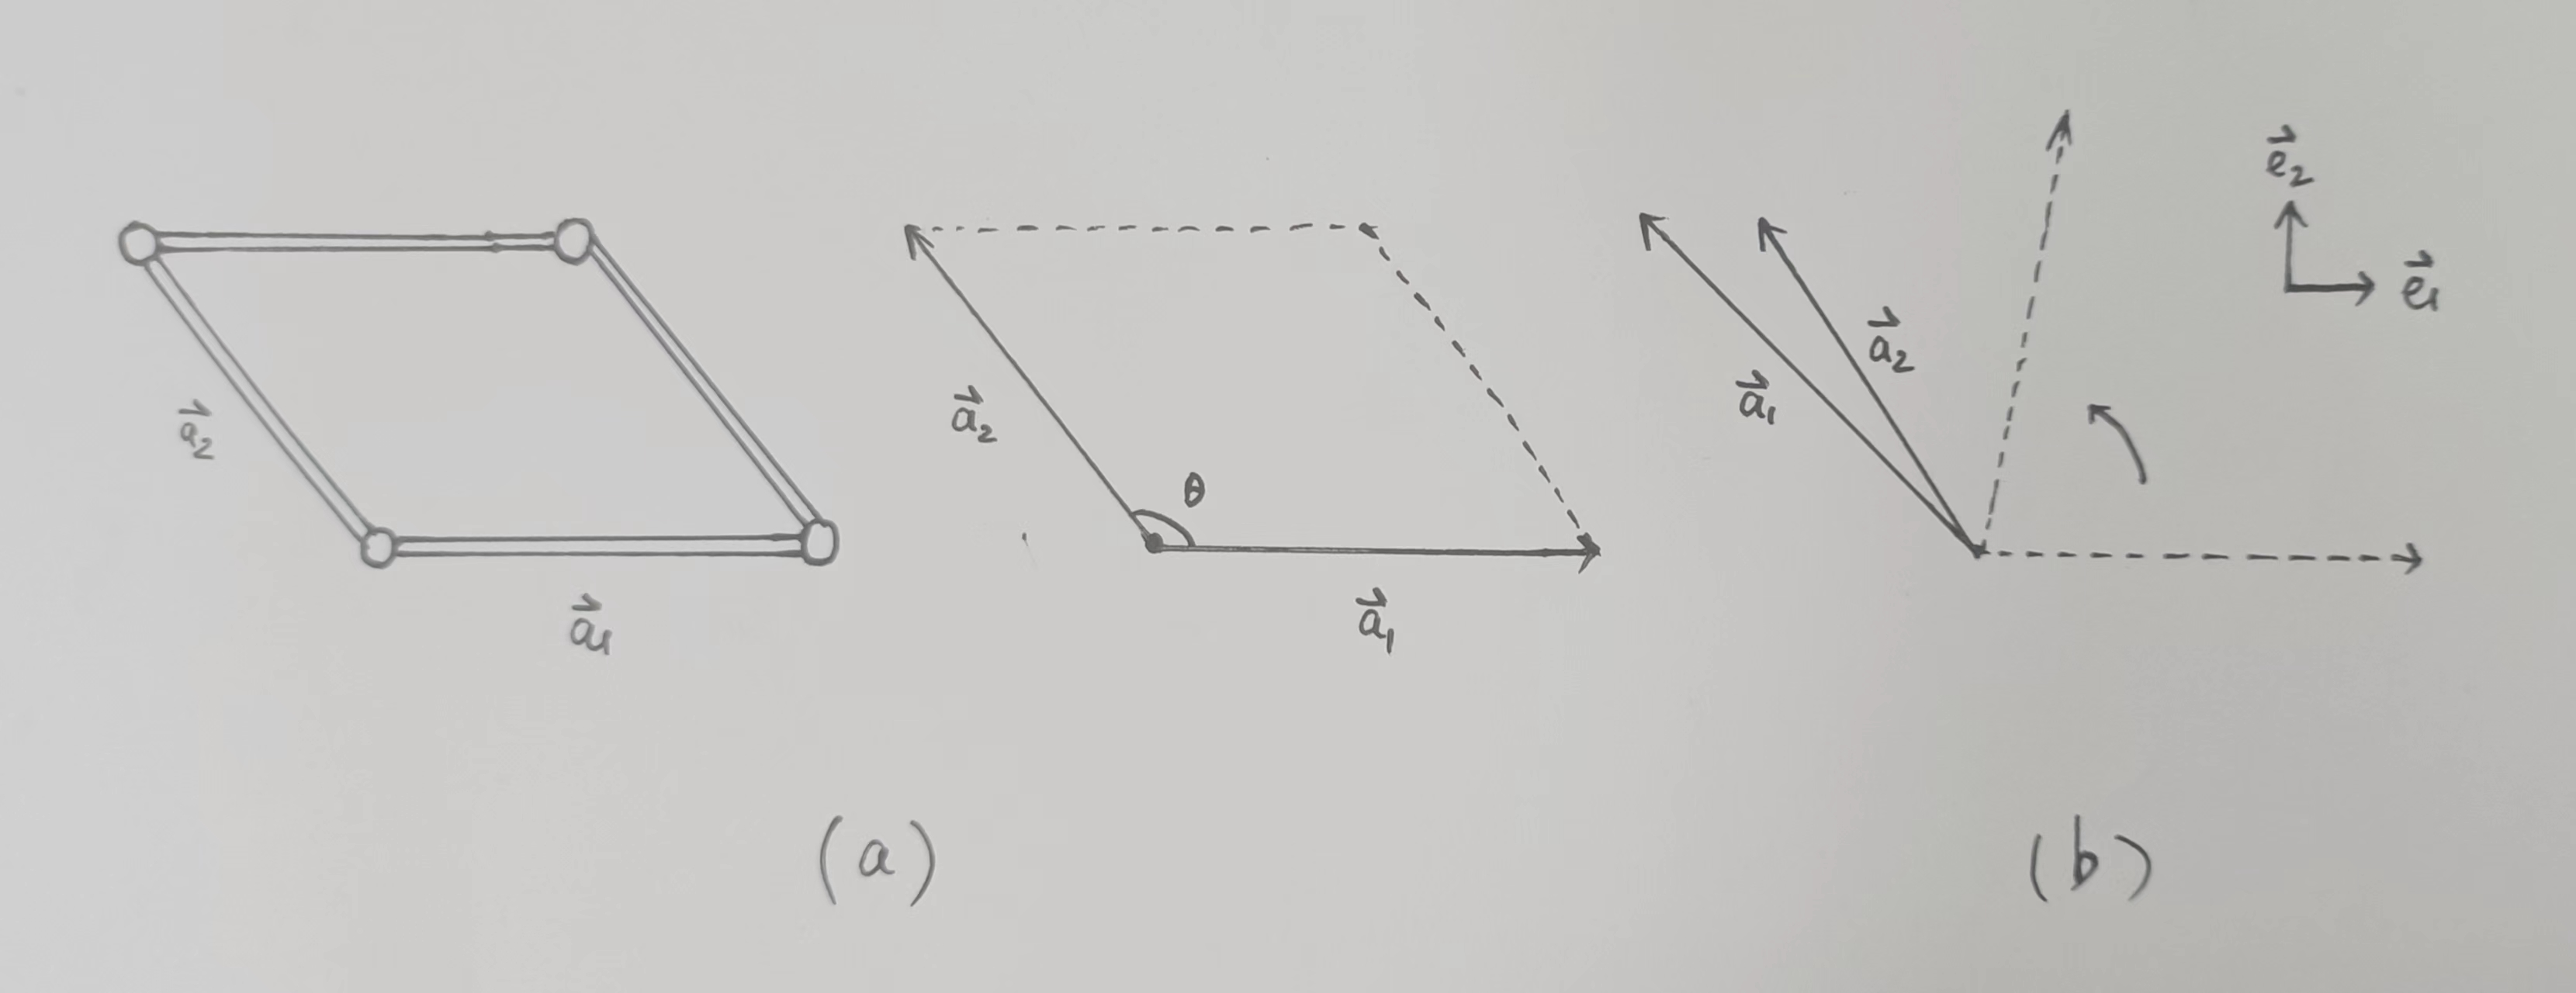
\includegraphics[width=0.8\textwidth]{figs_I1/1.jpg}
    \caption{Parallelogram and the Orientation}
    \label{fig:para_ori}
\end{figure}

\section{Determinant for Higher-order Matrices}
In the last part of analysis, we realize that the orientation is differentiated by whether the deformation of the image unit breaks the physical law (in the two-dimensional space). To place one edge to the opposite side of the other edge is illegal, or, to swap the position of the two edges is prohibited. Thus, without changing the sign of the determinant, we can arbitrarily change the angle of the two edges (namely, change the parallelogram into any shape), but we cannot change the positional relationship of the two edges. 

Now we look at the case when $n=3$ and 
$$ A = \begin{bmatrix}
    a_{11} & a_{12} & a_{13} \\
    a_{21} & a_{22} & a_{23} \\
    a_{31} & a_{32} & a_{33}
\end{bmatrix} = [\pmb{a}_1 \;\pmb{a}_2 \;\pmb{a}_3]\in\mathbb{R}^{3,3} $$
We just say that the shape of the image unit does not matter in the sign of $\det A$. Actually it does not matter for the volume (namely, the entire value of $\det A$) either, based on a fact we have all known in the primary school (see the figure \ref{fig:rectify_prism}). To rectify the tilted prism to an upright one is to add a vector in the bottom plain to the (tilted) height, thus we immediately obtain one of the basic properties of determinant:

\begin{figure}[H]
    \centering
    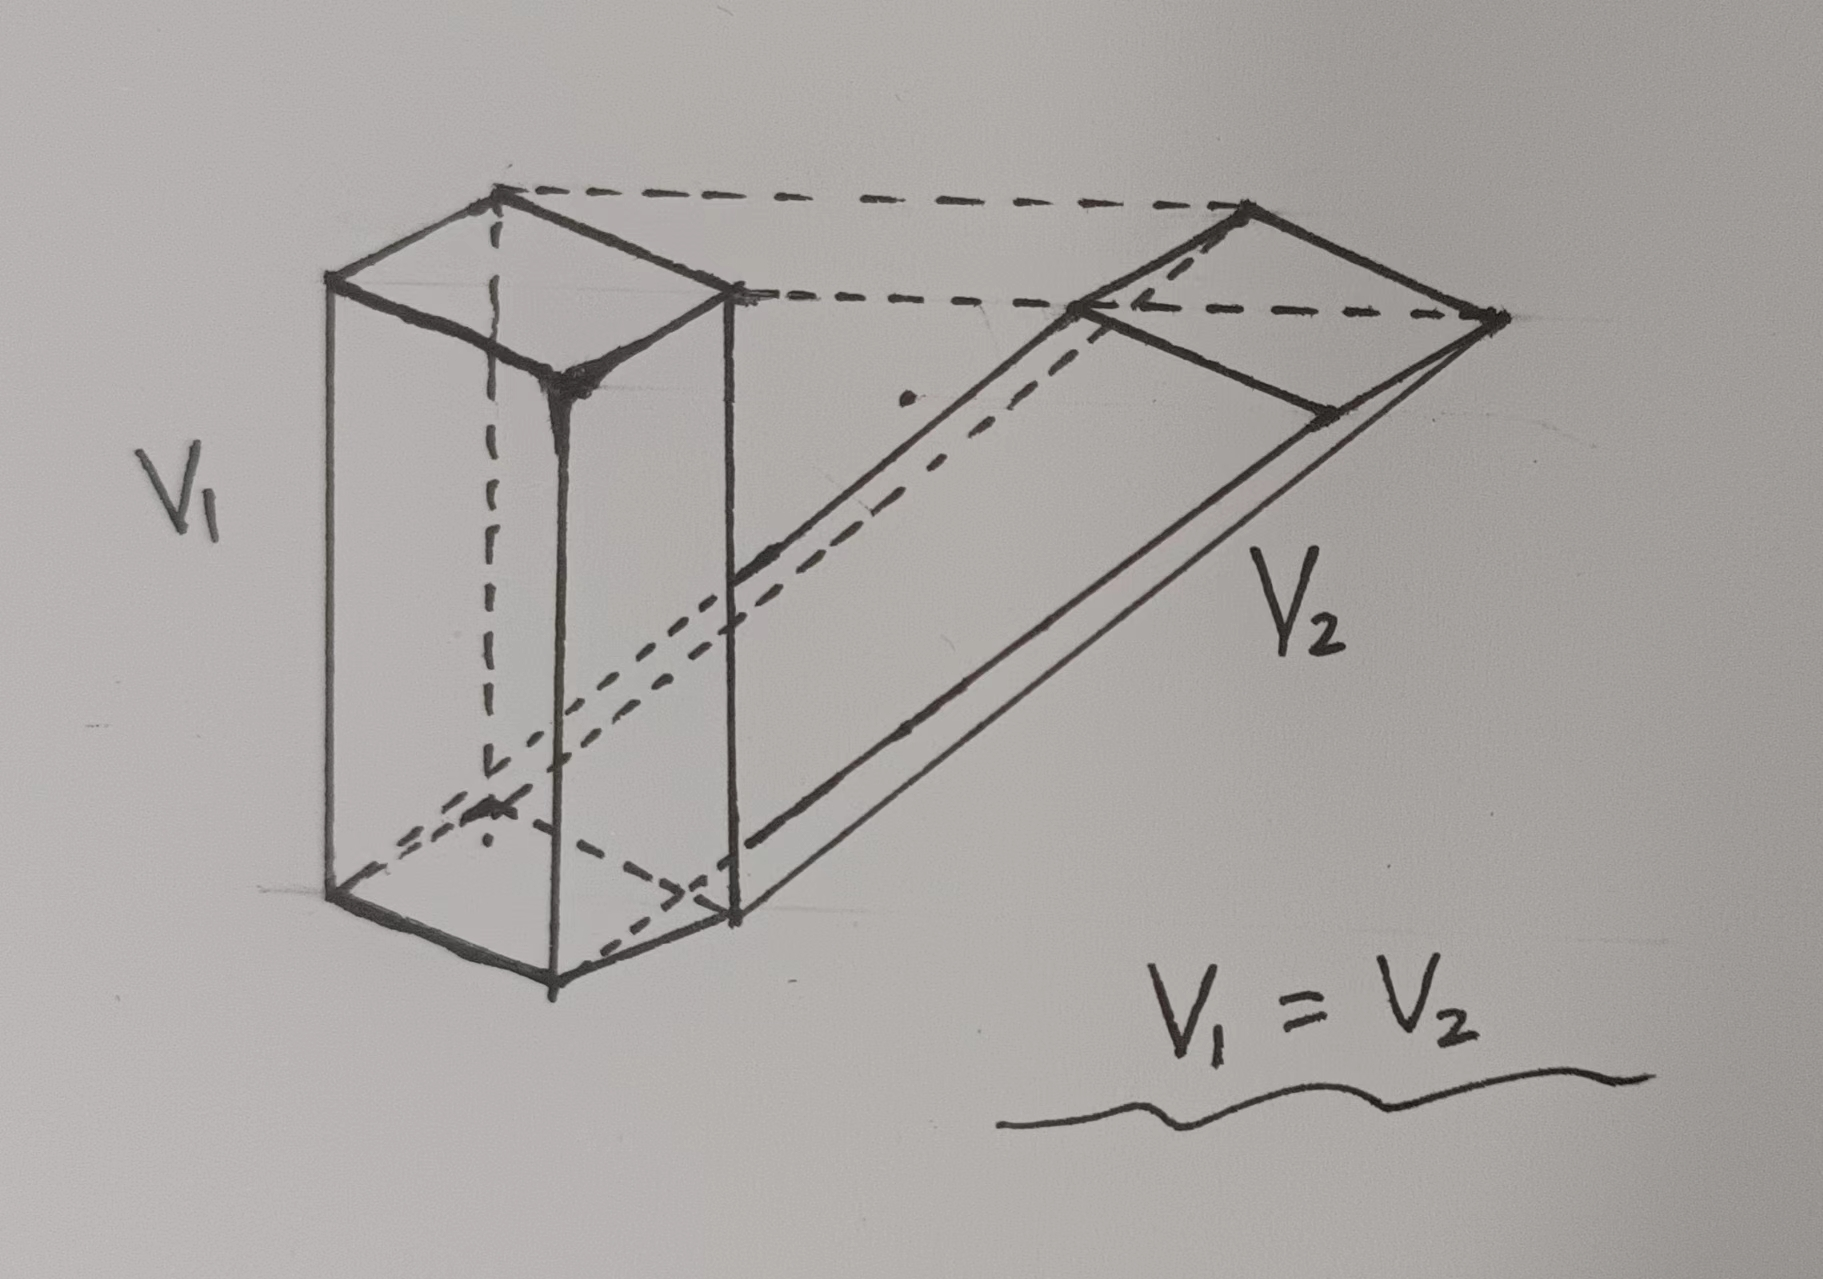
\includegraphics[width=0.8\textwidth]{figs_I1/2.jpg}
    \caption{Rectify the Tilted Prism}
    \label{fig:rectify_prism}
\end{figure}

\begin{Th}{Th\,8\_I1.1 nv}
    Adding a multiple of one column to another column does not change the determinant.
\end{Th}

Then in $\mathbb{R}^3$, we can enumerate all $3!=6$ possible positional relationships among the edges $\pmb{a}_1$, $\pmb{a}_2$ and $\pmb{a}_3$, assuming mutual orthogonality (see the figure \ref{fig:6_configs}). And the volume $V$ of the image unit, by Th \{, ID: 8\_I1.1\}, is (assume $a_{11}\neq 0$ without losing generality):
\begin{equation}
    \begin{aligned}
        V &= |\det A| = \left|\begin{array}{ccc}
        a_{11} & a_{12} & a_{13} \\
        a_{21} & a_{22} & a_{23} \\
        a_{31} & a_{32} & a_{33} 
    \end{array}\right| = \left|\begin{array}{ccc}
        a_{11} & 0 & 0 \\
        a_{21} & a_{22}-\frac{a_{12}}{a_{11}}a_{21} & a_{23}-\frac{a_{13}}{a_{11}}a_{21} \\
        a_{31} & a_{32}-\frac{a_{12}}{a_{11}}a_{31} & a_{22}-\frac{a_{13}}{a_{11}}a_{31} 
    \end{array}\right| \\
        &= |a_{11}|\times \text{abs} \left|\begin{array}{cc}
            a_{22}-\frac{a_{12}}{a_{11}}a_{21} & a_{23}-\frac{a_{13}}{a_{11}}a_{21} \\
            a_{32}-\frac{a_{12}}{a_{11}}a_{31} & a_{22}-\frac{a_{13}}{a_{11}}a_{31}
        \end{array}\right| \\
        &= | a_{11}a_{22}a_{33} - a_{11}a_{23}a_{32} - a_{12}a_{21}a_{33} + a_{12}a_{23}a_{31} + a_{13}a_{21}a_{32} - a_{13}a_{22}a_{31} |
    \end{aligned}
    \label{eq:abs_det_3}
\end{equation}

\begin{figure}[H]
    \centering
    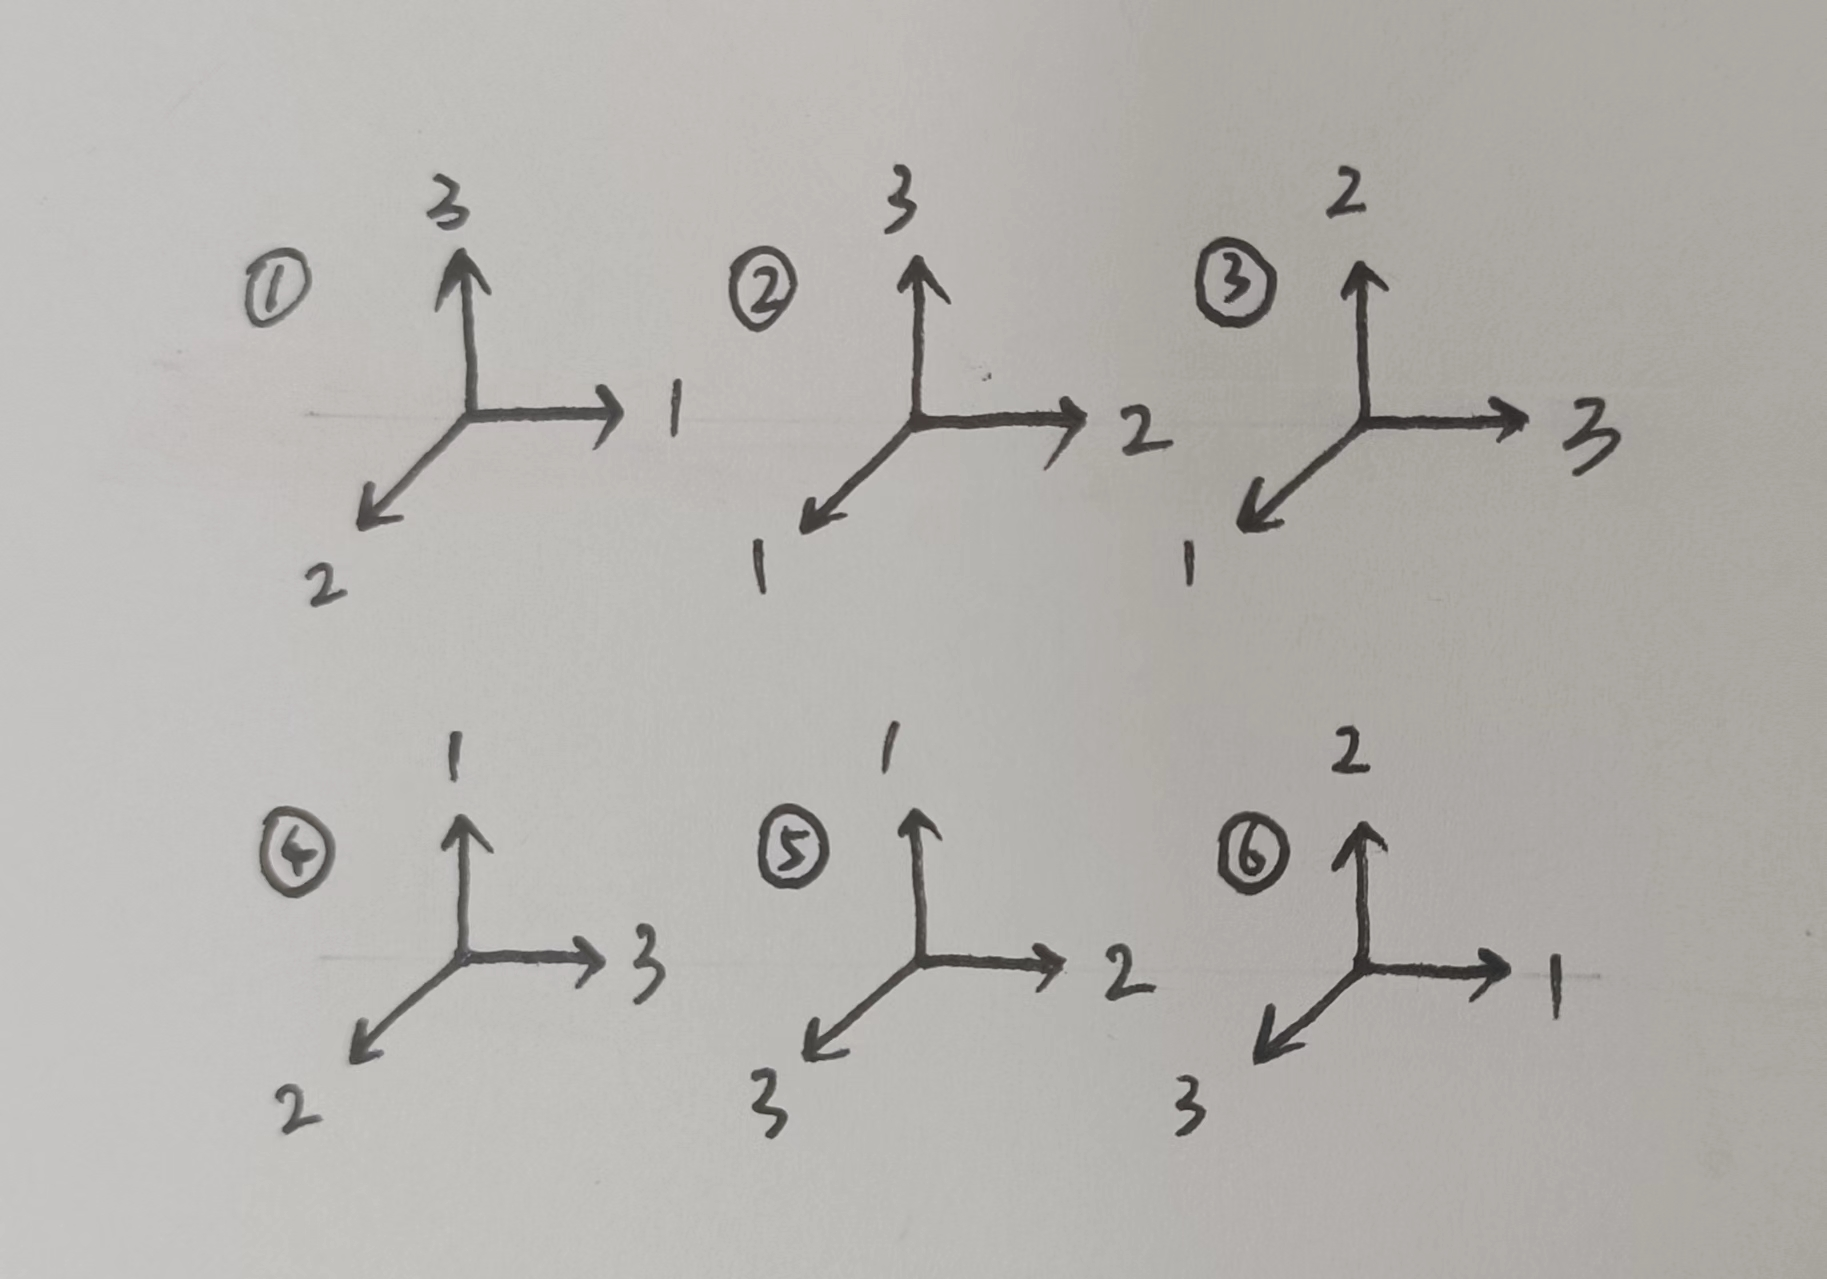
\includegraphics[width=0.8\textwidth]{figs_I1/3.jpg}
    \caption{Six Configurations}
    \label{fig:6_configs}
\end{figure}

To determine the sign of $\det A$ in the equation \ref{eq:abs_det_3}, let us inspect the 6 ``\textbf{configurations}'' in the figure \ref{fig:6_configs}. In this figure, each of the configurations (e.g. the configuration \textcircled{1}) is an orthogonal basis of $\mathbb{R}^3$, and each arrow represents the corresponding vector with the number marked (e.g. the arrow $1$ represents $\pmb{a}_1$). Imagine each configuration is a rigid ``frame'' in the 3D space, and we can rotate the frame in any direction. Then we find that some of the configurations are ``equivalent''. For example, the configuration \textcircled{1} can be rotated to coincide with the configuration \textcircled{3}, and the configuration \textcircled{2} can be rotated to coincide with the configuration \textcircled{4}. However, the configuration \textcircled{2} cannot coincide with the configuration \textcircled{3} by any rotation. If we say that the configurations that can be rotated to coincide with each other are ``equivalent'', then we can classify the 6 configurations into 2 equivalence classes: 
$$ (1) = (3) = (5) \neq (2) = (4) = (6). $$
Then this is, naturally for us, what the sign of $\det A$ reflects. 

Also, these 6 configurations are arranged in a order that: a configuration is obtained by a swap of two vectors from one of the adjacent configuration. For example, swapping $\pmb{a}_1$ and $\pmb{a}_2$ in \textcircled{1} gives \textcircled{2}, and swapping $\pmb{a}_2$ and $\pmb{a}_3$ in \textcircled{5} gives \textcircled{4}. Therefore, we get one of the basic properties of determinant.

\begin{Th}{Th\,8\_I1.2 nv}
    An odd number of swaps change the sign of $\det A$, while an even number of swaps does not.
\end{Th}

Back to the sign of $\det A$ in the equation \ref{eq:abs_det_3}, since the edges $\pmb{a}_1$, $\pmb{a}_2$ and $\pmb{a}_3$ must be one of the 6 configurations (in terms of the positional relationship), we can first associate the standard basis $(\pmb{e}_1, \pmb{e}_2, \pmb{e}_3)$ with one of the configurations — say, \textcircled{1} — and then determine the sign of $\det A$ according to which configuration $(\pmb{a}_1, \pmb{a}_2, \pmb{a}_3)$ belongs to. If $(\pmb{a}_1, \pmb{a}_2, \pmb{a}_3)$ belongs to \textcircled{1}, \textcircled{3} or \textcircled{5}, then $\det A>0$.

If you think it is still somewhat complex to figure out which configuration $A$ belongs to, here we use a analitical trick. If $A = [\pmb{a}_1\;\pmb{a}_2\;\pmb{a}_3]$ differs little from $I = [\pmb{e}_1\;\pmb{e}_2\;\pmb{e}_3]$ (i.e. each $\pmb{a}_i$ nearly coincides with $\pmb{e}_i$ in its direction), then $A$ is definitely of the configuration \textcircled{1}, with $\det A>0$. In this case, we can think that
$$ a_{ii} \gg 0; \qquad a_{ij}\approx 0 \quad (i\neq j). $$
Thus the equation \ref{eq:abs_det_3} is now
$$ 
\begin{aligned}
    0 < \det A = & \pm a_{11}a_{22}a_{33} \mp a_{11}a_{23}a_{32} \mp a_{12}a_{21}a_{33} \\
    & \pm a_{12}a_{23}a_{31} \pm a_{13}a_{21}a_{32} \mp a_{13}a_{22}a_{31} \\
    \approx & \pm a_{11}a_{22}a_{33} = a_{11}a_{22}a_{33},
\end{aligned}
$$
and the signs of other terms are decided accordingly:
\begin{equation}
    \det A = a_{11}a_{22}a_{33} - a_{11}a_{23}a_{32} - a_{12}a_{21}a_{33} + a_{12}a_{23}a_{31} + a_{13}a_{21}a_{32} - a_{13}a_{22}a_{31}. 
    \label{eq:det_A}
\end{equation}

Actually, here is another concise interpretation for \ref{eq:det_A}. Each term of the polynomial on the right side stands for the ``tendency'' or ``intensity'' of $A$ to belong to a corresponding configuration in the figure \ref{fig:6_configs}. For example, $a_{11}a_{22}a_{33}$ stands for the standard tendency, namely, the tendency of configuration \textcircled{1}, while $a_{11}a_{23}a_{32}$ stands for the configuration \textcircled{6}, which is obtained by swapping $\pmb{a}_2$ and $\pmb{a}_3$ from \textcircled{1}. If, similar to the ``analitical trick'' we just mentioned, only $a_{11}$, $a_{23}$ and $a_{32}$ are significantly positive, then $A$ is of the same configuration with $[\pmb{e}_1\;\pmb{e}_3\;\pmb{e}_2]$, which is the configuration obtained by swapping $\pmb{e}_2$ and $\pmb{e}_3$ from the standard one, namely, the configuration \textcircled{6}. Of course, the tendency of those ``positive-camp'' configurations should be assigned the positive sign, while those ``negative-camp'' vice versa.

Continued, as what we just talked about the tendency of the term $a_{11}a_{23}a_{32}$, it corresponds to the swap $\pmb{e}_2\leftrightarrow\pmb{e}_3$, which is identically reflected in its subscripts
$$ a_{11}a_{2\textcolor{red}{2}}a_{3\textcolor{red}{3}} \leftrightarrow a_{11}a_{2\textcolor{red}{3}}a_{3\textcolor{red}{2}} $$
Hence for such each term, the sign, the tendency, the parity of the permutation in its subscripts, are linked this way, which is the discussion of permutation, swap, parity in the note file all about.
\end{document}